% =================================================================
% RESEARCH PAPER MAIN MANUSCRIPT (v10.0)
% =================================================================
\documentclass[11pt,a4paper]{article}
\usepackage{iftex}
\ifXeTeX\else
  \PackageError{paper-template}{XeLaTeX is required}{Run xelatex; fontspec requires XeLaTeX.}
\fi
\usepackage{fontspec}
\IfFontExistsTF{Liberation Serif}{\setmainfont{Liberation Serif}}{\setmainfont{Times New Roman}}
\usepackage{graphicx}
\usepackage{amsmath,amssymb,amsfonts}
\usepackage[a4paper, margin=1in]{geometry}
\usepackage{setspace}
\setstretch{1.15}
\usepackage[numbers,sort&compress]{natbib}
\setlength{\bibsep}{3.5pt plus 1pt minus 1pt}
\setlength{\emergencystretch}{4em}
\usepackage{booktabs}
\usepackage{microtype}
\usepackage{xcolor}
\usepackage{enumitem}
\usepackage{array}
\usepackage{tabularx}
\usepackage{multirow}
\usepackage{xurl}
\usepackage[hidelinks,unicode=true]{hyperref}
\urlstyle{same}
\providecommand{\doi}[1]{\href{https://doi.org/#1}{doi:\nolinkurl{#1}}}
\usepackage{caption}
\usepackage{subcaption}
\usepackage{placeins}
\captionsetup{
  font=small,
  labelfont=bf,
  textfont=normalfont,
  labelsep=period,
  justification=justified,
  singlelinecheck=true,
  skip=6pt
}
\setlength{\textfloatsep}{14pt plus 2pt minus 2pt}
\setlength{\floatsep}{12pt plus 2pt minus 2pt}
\setlength{\intextsep}{12pt plus 2pt minus 2pt}
\setcounter{topnumber}{4}
\setcounter{bottomnumber}{3}
\setcounter{totalnumber}{6}
\renewcommand{\topfraction}{0.88}
\renewcommand{\bottomfraction}{0.80}
\renewcommand{\textfraction}{0.10}
\renewcommand{\floatpagefraction}{0.70}

\usepackage{fancyhdr}
\setlength{\headheight}{14pt}
\pagestyle{fancy}
\fancyhf{}
\fancyhead[L]{\small\nouppercase{\leftmark}}
\fancyhead[R]{\small\thepage}
\renewcommand{\headrulewidth}{0.4pt}
\fancypagestyle{plain}{
  \fancyhf{}
  \fancyfoot[C]{\small\thepage}
  \renewcommand{\headrulewidth}{0pt}
}
\renewcommand{\sectionmark}[1]{\markboth{\thesection\quad #1}{}}

\usepackage{newunicodechar}
\newunicodechar{δ}{\ensuremath{\delta}}
\newunicodechar{Γ}{\ensuremath{\Gamma}}

\title{\textbf{Partial Identification and Simultaneous Rank Inference for Pathogen Hospitalization Comparisons among Reported Foodborne Outbreak Cases, United States, 2009--2023}}
\author{Chi Wang}
\date{November 27, 2026}

\begin{document}
\maketitle
\normalfont\mdseries

\begin{abstract}
\noindent Surveillance comparisons of pathogen hospitalization rely on unexamined denominator conventions for unrecorded outcomes and overlook clustering and multiplicity. We estimated standardized hospitalization proportions among \textit{reported outbreak cases} (rather than intrinsic pathogen virulence) across 4,133 confirmed foodborne outbreaks in the US National Outbreak Reporting System (2009--2023), restricted to 12 shared setting--period cells (3,176 outbreaks; 72,132 cases; 90.4\% of weight in 2009--2018). Without assumptions on unrecorded hospitalization outcomes, 4 of 15 sample pairs separated (Shiga toxin--producing \textit{Escherichia coli} [STEC] above \textit{Campylobacter}, \textit{Clostridium perfringens}, and norovirus GI and GII). Nominal outbreak-clustered ($p = 0.024$) and exposure-state-clustered ($p = 0.033$) tests placed STEC above norovirus GII, whereas primary studentized bootstrap-$t$ inference rejected zero of 30 one-sided hypotheses ($p = 0.249$; all 95\% ranks $[1,6]$); thus worst-case statistical support is fragile and method-dependent. Within-cell hospitalization was higher in partially than fully recorded outbreaks ($+0.05$ to $+9.02$ percentage points [pp]), though STEC showed negative standardized observed-versus-full ($-2.53$ pp) and multistate ($-1.28$ pp) contrasts. Under bounded missingness departures anchored to external surveillance benchmarks, simultaneous 95\% ranks separated STEC $[1,1]$, \textit{Salmonella} $[2,2]$ and \textit{Campylobacter} $[3,3]$ above $[4,6]$ up to a joint studentized bootstrap-$t$ breakdown deviation of 11.6 pp (13.5 pp for \textit{Campylobacter}; 7.9 pp under the worst-case critical value), whereas lower-tier orderings failed below 5 pp.

\vspace{0.5em}\noindent\textbf{Keywords:} foodborne disease outbreaks; hospitalization; partial identification; breakdown frontiers; rank confidence sets
\end{abstract}

\section{Introduction}\label{sec:intro}

Foodborne outbreak surveillance in the United States is a primary national source on how frequently illnesses associated with specific enteric pathogens result in hospitalization. Since 2009, state, local and territorial health departments have reported outbreaks across transmission modes to the National Outbreak Reporting System (NORS)~\cite{hall2013acute}. Descriptive summaries routinely compare pathogens by reported hospitalization percentages: in enteric outbreaks during 2009--2019, reported hospitalization was 20.9\% for \textit{Salmonella} and 22.8\% for \textit{Escherichia coli} outbreaks versus 2\% for norovirus outbreaks~\cite{wikswo2022enteric}, and annual surveillance reports tabulate hospitalization percentages alongside etiology~\cite{cdc2026surveillance2019}. Outbreak hospitalization metrics also enter composite severity indices~\cite{simpson2022analysing} and inform national burden estimates, for some pathogens serving as the sole empirical source~\cite{scallanwalter2025foodborne}.

For each outbreak, NORS records the estimated number of ill persons, the number hospitalized and, separately, the number of ill persons with known hospitalization status~\cite{cdc2014norsguidance}. The difference between total illnesses and persons with known status represents cases with unrecorded hospitalization outcomes rather than confirmed non-hospitalized cases. Published analyses resolve these unrecorded cases by convention: dividing hospitalizations by all ill persons implicitly treats every unrecorded case as not hospitalized~\cite{heiman2015escherichia,cdc2026surveillance2019}, whereas dividing by persons with known status assumes that unrecorded cases were hospitalized at the same rate as recorded cases~\cite{burke2019norovirus}. Although prior audits have examined field-level completeness in NORS~\cite{zhang2022evaluating} and demonstrated that structural missingness can bias derived outbreak metrics~\cite{diemer2024missingness}, neither the impact of unrecorded outcomes on pairwise pathogen rankings nor the joint statistical inference required when outbreak clustering, estimated standardization weights and multiple testing are present has been quantified.

Comparisons across pathogens face two further methodological challenges. First, pathogen groups occur in distinct food-preparation settings that independently predict severe outcomes~\cite{burke2019norovirus}, while state reporting intensity varies substantially~\cite{white2022foodborne} and shifted during the COVID-19 pandemic~\cite{ray2021decreased}; crude hospitalization percentages therefore conflate pathogen differences with setting and period mix. Second, cases cluster strongly within outbreaks whose sizes are heavily right-skewed: ignoring outbreak clustering or treating sample worst-case intervals as deterministic ignores sampling variability, whereas standardizing to a pooled reference distribution introduces dependence across groups through shared estimated weights.

To address these gaps simultaneously, we developed an integrated partial-identification and stacked M-estimation inference framework~\cite{manski1989anatomy,horowitz2000nonparametric,keiding2014standardization,ratitch2013missing,stefanski2002calculus,imbens2004confidence,romano2005exact} for six major foodborne pathogen groups in NORS during 2009--2023: \textit{Salmonella}, Shiga toxin--producing \textit{E. coli} (STEC), \textit{Campylobacter}, \textit{Clostridium perfringens}, norovirus genogroup I (GI) and norovirus genogroup II (GII). Beyond characterizing sample worst-case bounds and tipping points, we derive outbreak-cluster sandwich covariances that couple reference-weight uncertainty with within-cell sampling variance, construct Imbens--Manski uniformly valid 95\% confidence intervals and stepdown family-wise error rate (FWER) adjusted confidence tipping points across all 15 pairwise comparisons, diagnose outbreak-size concentration, and propose a Value-of-Information (VoI) follow-up allocation rule validated by retrospective masking on complete-status NORS outbreaks.

\section{Methods}\label{sec:methods}

\subsection{Data Source, Record Audit and Common Support}\label{sec:data}

We conducted a cross-sectional analysis of outbreak-level records in the public CDC NORS dataset~\cite{cdc2024norsdata}, downloaded on 25 November 2026 (portal rows last updated 20 December 2024), adhering to RECORD reporting standards~\cite{benchimol2015record} (full checklist in Supplementary Section S4 / Table S12). Across NORS reporting revisions spanning 2009--2023~\cite{cdc2014norsguidance,wikswo2022enteric}, the core variables---estimated total primary ill persons (\texttt{Illnesses}, $C_i$), hospitalizations ($H_i$), and persons with known hospitalization status ($K_i$)---retain consistent definitions~\cite{cdc2014norsguidance,cdc2024norsdata}. As documented in CDC NORS guidance~\cite{cdc2014norsguidance} (pp.~15--16), $C_i$ combines total ill persons ``including lab-confirmed and probable cases'' based on case definitions or estimates, so $M_i = C_i - K_i$ mixes individually ascertained cases lacking hospitalization records with estimated cases (analogous to ``missing types''~\cite{jiang2018using}); because the public NORS extract does not separate confirmed, probable and estimated counts, missing-type bound-tightening would require restricted data. Reporting by health departments is voluntary~\cite{hall2013acute}, and etiologies are classified as confirmed or suspected~\cite{cdc2026surveillance2019}. Eligible primary outbreaks had food as primary mode, began in 2009--2023, and had confirmed etiology in one of six study groups: any \textit{Salmonella} serotype, STEC, any \textit{Campylobacter} species, \textit{C. perfringens}, norovirus GI or norovirus GII (single or same-group multi-entry~\cite{cdc2014norsguidance}; single-entry~\cite{weller2026single}, confirmed O157-restricted STEC~\cite{tack2021shiga} [279/388 outbreaks], and excluding 6 \textit{Salmonella} serovar Typhi outbreaks [87 cases, 42 hospitalized] in sensitivity analyses). Excluded groups comprised 951 suspected study-group outbreaks (included in variant R8), 304 confirmed norovirus outbreaks lacking genogroup (only 2 recoverable from recorded genotype tokens; included in R7b), and 300 mixed/non-study outbreaks (104 with $\ge 1$ confirmed study group; Supplementary Table S2).

Complete-field consistent records satisfied $0 \le H_i \le K_i \le C_i$ with both $H_i$ and $K_i$ recorded (3,976 outbreaks), whereas \textit{fully recorded outbreaks} denote zero unrecorded cases ($M_i = 0$; 2,414 outbreaks in common support). Incomplete records were retained under logical bounds (Supplementary Table S1): blank $K_i$ set $K_{\text{eff},i} = H_i$ (leaving $C_i - H_i$ unrecorded); blank $H_i$ with $K_i = 0$ implied $H_i = 0$; and blank $H_i$ with $K_i > 0$ (23 outbreaks), or both fields blank, set $K_{\text{rec},i} = 0$ and treated all $C_i$ cases as unrecorded (in the 23 blank-$H$, $K_i > 0$ outbreaks, this discards $H_i \le K_i$ harmlessly for worst-case validity while preventing point-rate distortion). Contradictions ($H_i > C_i$ or $K_i > C_i$) or $C_i \le 0$ were excluded.

Seven harmonized settings---restaurant, catering/banquet, private home, institution, other, multiple and unknown (Supplementary Section S1)---were crossed with three periods (2009--2013, 2014--2018, 2019--2023). The primary analysis restricted attention to the data-selected common support of cells with $\ge 3$ outbreaks per group and directly standardized all six groups~\cite{keiding2014standardization} to pooled-case weights $w_s = C_{\cdot s} / \sum_{s'} C_{\cdot s'}$. Under pooled-case weighting, the standard population draws 72.8\% (52,507 of 72,132 cases) from \textit{Salmonella} and norovirus GII, so $\theta_j$ reflects hospitalization under that empirical case mix. All inference is conditional on this selected support; we also evaluated support thresholds $\ge 2$ (R4a) and $\ge 5$ (R4b), period-only standardization (R2), equal within-cell outbreak weighting (R10, normalizing both outbreak $H_i/C_i$ and known-status $H_{\text{rec},i}/K_{\text{rec},i}$ counts per outbreak), alternative external weights (R6a--c), healthcare/LTCF exclusion (R9), and single-state-only restriction (R11).

\subsection{Target Estimand, Worst-Case Bounds and Breakdown Frontiers}\label{sec:bounds}

For group $j$ and cell $s$, let $C_{js}$, $H_{js}$, $M_{js}$, $H_{\text{rec},js}$, and $K_{\text{rec},js}$ denote cell sums of $C_i$, $H_i$, $M_i$, and recorded-status counts ($H_{\text{rec},i} = H_i, K_{\text{rec},i} = K_{\text{eff},i}$ for consistent records; $0, 0$ when $H_i$ is blank and $K_i > 0$ or both are blank). The target estimand is the case-weighted directly standardized hospitalization proportion among \textit{reported foodborne outbreak cases}:
\begin{equation}
  \theta_j = \sum_s w_s \, \frac{H_{js} + H^{u}_{js}}{C_{js}},
  \label{eq:theta}
\end{equation}
where $H^{u}_{js} \in [0, M_{js}]$ is unobserved hospitalizations among unrecorded cases. All bounds take the estimated case counts $C_i$ and reported counts $(H_i, K_i)$ as exact; differential case ascertainment is not bounded here (\S\ref{sec:limitations}). Without assumptions on unrecorded hospitalization outcomes~\cite{manski1989anatomy}, $\theta_j$ lies in $[L_j, U_j]$:
\begin{equation}
  L_j = \sum_s w_s \frac{H_{js}}{C_{js}}, \qquad
  U_j = \sum_s w_s \frac{H_{js} + M_{js}}{C_{js}}.
  \label{eq:bounds}
\end{equation}
Pair $(h, l)$ separates in the sample without outcome assumptions if $L_h > U_l$~\cite{horowitz2000nonparametric}. Let $p_{js} = H_{\text{rec},js}/K_{\text{rec},js}$ be the within-cell recorded rate ($\delta = 0$ assumes within-cell missingness at random, MAR). Motivated by bounded-variation partial identification~\cite{manski2018how}, we evaluated:
\begin{enumerate}
  \item \textit{Additive bounded-variation bands and breakdown points:} allowing each cell's unrecorded rate in $[p_{js} - \delta_{\text{down}},\, p_{js} + \delta_{\text{up}}] \cap [0, 1]$~\cite{ratitch2013missing,liublinska2014sensitivity}:
  \begin{equation}
  \begin{aligned}
    L_j(\delta_{\text{down}}) &= \sum_s w_s \frac{H_{js} + M_{js}\max(0,\, p_{js} - \delta_{\text{down}})}{C_{js}}, \\
    U_j(\delta_{\text{up}}) &= \sum_s w_s \frac{H_{js} + M_{js}\min(1,\, p_{js} + \delta_{\text{up}})}{C_{js}},
  \end{aligned}
    \label{eq:delta}
  \end{equation}
  where symmetric $\delta_{\text{down}} = \delta_{\text{up}} = \delta$ recovers worst-case $[L_j, U_j]$ at $\delta = 100\text{ pp}$. For the 52 blank-$K_i$ outbreaks (2.3\% of eligible cases; true $K_i \in [H_i, C_i]$), setting $K_{\text{eff},i} = H_i$ is exact for worst-case bounds and conservative for the $\delta$-upper bound; a strictly conservative $\delta$-lower bound holding $H_i$ fixed is verified in sensitivity checks. Sample breakdown points $\delta^{*}_{hl} = \inf\{\delta \ge 0 : L_h(\delta) \le U_l(\delta)\}$~\cite{kline2013sensitivity,masten2020inference} were solved analytically (Supplementary Section S2), alongside 2D breakdown frontiers $(\delta_{h,\text{down}}, \delta_{l,\text{up}})$ and asymmetric $-10/+5, -15/+5, -20/+5\text{ pp}$ plus diagnostic-informed group-specific asymmetric bands (\textit{Salmonella} $-10/+5\text{ pp}$, \textit{Campylobacter} $-7/+5\text{ pp}$, others $\pm 5\text{ pp}$). We use the additive scale as our primary target because public-health policy and case-burden comparisons depend on absolute hospitalization risk differences rather than relative odds ratios across groups spanning 0.5\% to 28.5\%; we anchor $\delta$ externally against US per-case benchmarks~\cite{scallan2011foodborne,scallanwalter2025foodborne} and low-missingness states, and also check outbreak-level MAR (R13) and common-mechanism scaling $q_{js} = \min(1, \alpha p_{js})$ (Supplementary Fig.~S4).
  \item \textit{Odds-ratio (OR) pattern-mixture scale:} bounding unrecorded odds in $[\text{odds}(p_{js})/\Gamma,\, \Gamma\cdot\text{odds}(p_{js})]$ ($\Gamma \ge 1$) with sample critical breakdown $\Gamma^{*}_{hl}$, alongside a $0.1\%$ continuity floor ($p_{js} = 0.001$) on 9 zero-rate cells and formal 30-hypothesis inference ($\Gamma = 1.5, 2, 3, 5$ and $\Gamma^{*}_{0.95}$).
  \item \textit{Denominator contamination and selection sensitivity:} drawing on contaminated-data bounds~\cite{horowitz1995identification,molinari2008partial}, we added variants treating 25\% of unrecorded cases as extrapolated non-cases ($C'_i = C_i - 0.25 M_i$, R14a) and a selection-sensitivity variant restricting to outbreaks with $\le 50\%$ unrecorded status ($M_i/C_i \le 0.50$, R14b).
  \item \textit{Composition-adjusted partial vs.\ full diagnostics:} comparing known-status rates between partially ($M_i > 0, K_{\text{rec},i} > 0$) and fully ($M_i = 0$) recorded outbreaks crudely, across shared cells containing both partially and fully recorded outbreaks (within-cell difference and common-cell standardized observed-minus-full difference, $\theta^{\text{cc}}_j(0) - r^{\text{cc}}_{\text{full},j}$, evaluated over identical shared cells and weights), stratified by single-state vs.\ multistate status, and descriptively in 11 high-completeness states satisfying both $<5\%$ unrecorded cases and $\ge 200$ common-support cases (Wilson 95\% CIs).
\end{enumerate}

\subsection{Superpopulation Target, 30-Hypothesis Inference and Double-Bootstrap Evaluation}\label{sec:inference}

Although NORS approaches a national census of reported outbreaks in a fixed historical window, statistical inference treats the observed outbreaks in each cell as an independent stratified draw from a superpopulation of foodborne outbreak-generation and reporting conditional on the selected common support~\cite{keiding2014standardization}. This working assumption ignores cross-outbreak correlation (which we examine directly via exposure-state clustering, CV3 jackknife, and Bayesian cluster resampling below); hierarchical shrinkage~\cite{normand1997statistical} is a complementary approach for sparse cells.

For all $30$ one-sided hypotheses $H_{0,(h,l)}: \theta_h \le \theta_l$ (both directions of all 15 pairs, avoiding data-selected testing~\cite{andrews2024inference} and framing inference on many one-sided moment inequalities~\cite{chernozhukov2019inference}), each lower difference $\Delta^{L}_{hl} = L_h - U_l$ is smooth away from kinks at $p_{js} = \delta$ or $1 - \delta$ (0 of 72 cells lay within $10^{-6}$ of kinks at $\delta = 5\text{ pp}$; minimum distance across all finite 95\% roots was $0.0013\text{ pp}$ under CV3, $0.0024\text{ pp}$ under HC1, and $0.0056\text{ pp}$ under bootstrap-$t$; estimators at kinks can exhibit non-Gaussian directional limits~\cite{fang2019inference,masten2020inference}). Outbreak-HC1 sandwich covariances $\widehat{V}_{\text{HC1}}$ (Eq.~\ref{eq:sandwich}) matched closed-form influence functions $\psi_i$ to $\le 1.64 \times 10^{-12}$ (worst case), $2.92 \times 10^{-13}$ ($\delta = 5\text{ pp}$), and $4.00 \times 10^{-13}$ ($-15/+5\text{ pp}$), while OR ($\le 6.40 \times 10^{-13}$) and group-specific asymmetric ($\le 3.16 \times 10^{-13}$) influence functions matched central-difference covariances and vectorized bootstrap-$t$ expansions agreed to $\le 5.6 \times 10^{-17}$ on $\Delta^L$ and $\le 6.9 \times 10^{-18}$ on standard errors:
\begin{equation}
  \widehat{V}_{\text{HC1}} = \sum_{j=1}^{G}\sum_{s=1}^{K} \widehat{J}_{js}\, \widehat{\Omega}_{js}^{\text{HC1}}\, \widehat{J}_{js}^{\top}, \qquad
  \widehat{\Omega}_{js}^{\text{HC1}} = \frac{1}{n_{js}(n_{js} - 1)} \sum_{i \in (j, s)} (Z_i - \bar{Z}_{js})(Z_i - \bar{Z}_{js})^{\top}.
  \label{eq:sandwich}
\end{equation}
Because NORS's exposure-state field comprises 52 single jurisdictions plus a CDC-coordinated Multistate category (219 outbreaks), we formed 53-cluster exposure-state CV1 covariances $\widehat{V}_{\text{state}}$, computed each cluster's share of total score variance $s_g = \|\Phi_g\|_2^2 / \sum \|\Phi_{g'}\|_2^2$ and plug-in effective cluster count $G_{\text{eff}} = 1/\sum s_g^2$~\cite{carter2017asymptotic,mackinnon2023cluster} (noting that plug-in $G_{\text{eff}}$ from stacked influence scores approximates the scalar variance-ratio effective cluster count of~\cite{carter2017asymptotic,mackinnon2023cluster}), and added three cluster-robust checks less vulnerable to a dominant cluster: (i) leave-one-cluster-out \textbf{CV3 jackknife} variances~\cite{mackinnon2023cluster} (all 53/53 and 52/52 leave-cluster-out tables valid), (ii) a \textbf{Bayesian 53-cluster bootstrap-$t$} drawing i.i.d.\ $\text{Exp}(1)$ cluster weights ($B = 2,000$), and (iii) splitting Multistate into 219 singleton clusters (271 clusters) alongside full inference within the 52 single states of variant R11.

Recognizing that severe outbreak skewness and small cells ($N_{\text{eff}} \approx 2$) distort asymptotic Gaussian critical values and standard cluster approximations~\cite{cameron2008bootstrap,mackinnon2017wild,canay2021wild,mackinnon2023cluster}, we evaluated six 30-hypothesis stepdown Max-$T$ procedures~\cite{romano2005exact} without claiming formal pre-specification: (1) outbreak-HC1 Gaussian (200,000 multiplier draws), (2) 53-cluster exposure-state CV1 Gaussian, (3) 53-cluster CV3 jackknife Gaussian, (4) 9,999-draw unrestricted Rademacher wild cluster bootstrap (WCB), (5) Bayesian 53-cluster bootstrap-$t$ ($B = 2,000$), and (6) outbreak-stratified replicate-studentized bootstrap-$t$ ($T^{(b)}_m = (\Delta^{L,(b)}_m - \widehat{\Delta}^L_m)/\widehat{\sigma}_{\text{HC1},m}^{(b)}$, $B = 2,000$, zero degenerate SE entries). Pointwise Imbens--Manski~\cite{imbens2004confidence} 95\% intervals are also reported with explicit finite-sample under-coverage caveats~\cite{stoye2009more}.

Simultaneous 95\% rank confidence sets $[1 + m^{-}_j,\, G - m^{+}_j]$ count the number of competitors rejected significantly above ($m^{-}_j$) and significantly below ($m^{+}_j$) group $j$ at family-wise $\alpha = 0.05$; these rank intervals are valid and conservative under partial identification because $\theta_h - \theta_l \ge \Delta^L_{hl}$ across the identified set~\cite{klein2020joint,mogstad2024inference} (partitioning methods~\cite{almohamad2021simultaneous,almohamad2022simultaneous} can shorten intervals for small $G = 6$ under point identification). Following~\cite{kline2013sensitivity,masten2020inference}, scalar statistical breakdown points $\delta^{*}_{0.95}$ and $\Gamma^{*}_{0.95}$ are inverse one-sided lower confidence bounds tested pointwise in $\delta$ or $\Gamma$ using fixed-level critical values ($c(\delta)$ from a 21-point grid for Gaussian procedures and 14-point grid for $c_{\text{bt}}(\delta)$, with all finite bootstrap-$t$ roots refined by exact uninterpolated $c_{\text{bt}}(\delta)$ evaluation to residual $\le 3.1 \times 10^{-5}$ and unique crossings verified on a 201-point scan; simultaneous confidence bands over the 2D frontiers in Fig.~4 would require a uniform band~\cite{masten2020inference}). To evaluate empirical 30-test FWER non-circularly under the least-favourable boundary null ($\Delta^L_{hl} = 0$), we conducted both a \textbf{stratified outbreak double bootstrap}~\cite{beran1988prepivoting} ($400$ outer worlds $\times 499$ inner resamples preserving $n_{js}$; no state correlation simulated) and a \textbf{53-cluster Bayesian double bootstrap} ($300$ outer $\text{Exp}(1)$ cluster-weighted worlds $\times 399$ inner draws simulating exposure-state and Multistate dependence), re-estimating every procedure's critical value inside each outer world. Finally, we evaluated 30-test inference under R2, R10, R4a/R4b, diagnostic-informed asymmetric bands, and exact leave-one-outbreak-out (LOO, all 3,176 outbreaks) and leave-largest-outbreak-out (LLO) deletions, alongside exploratory non-response follow-up simulations~\cite{hansen1946problem} (Supplementary Section S2, Tables S5--S11).

\section{Results}\label{sec:results}

\subsection{Study Population, Record Audit, Excluded Categories and Common Support}\label{sec:res-cohort}

Among 66,713 NORS outbreak records, 11,358 were foodborne outbreaks in 2009--2023, of which 4,133 outbreaks (103,040 cases) had confirmed etiology in one of six study groups: \textit{Salmonella} (1,758 outbreaks; 47,779 cases), norovirus GII (1,206; 29,712), STEC (388; 5,818), norovirus GI (297; 7,998), \textit{Campylobacter} (296; 3,254) and \textit{C. perfringens} (188; 8,479) (Figure~\ref{fig:flow}). Overall, 3,908 eligible outbreaks had a single etiology entry and 225 had multiple entries within one group. Auditing found zero arithmetic contradictions; 3,976 outbreaks (95,781 cases) were complete-field consistent and 157 (7,259 cases) had blank outcome fields (52 blank $K_i$, 28 blank $H_i$ with $K_i=0$, 23 blank $H_i$ with $K_i>0$, and 54 both blank; Supplementary Table S1), leaving 19.4\% of eligible cases with unrecorded status.

Three excluded foodborne groups were profiled separately (Supplementary Table S2): 951 suspected study-group outbreaks (12,965 cases; median 6 [IQR 3--14]; recorded hospitalization 1.8\%; unrecorded status 13.5%), 304 confirmed norovirus outbreaks lacking genogroup specification (7,679 cases; median 16 [8--28]; 1.0\% hospitalized; 20.6\% unrecorded), and 300 mixed or non-study multi-agent outbreaks (8,480 cases; 4.0\% hospitalized; 15.8\% unrecorded; including 104 with $\ge 1$ confirmed study group, 4,541 cases). Twelve of 21 setting--period cells met the common-support threshold ($\ge 3$ outbreaks per group), retaining 3,176 outbreaks (76.8\%) and 72,132 cases (70.0\%; 61.0\% for \textit{Salmonella} and 67.8\% for STEC to 77.5\%--81.3\% for the other four groups; Supplementary Table S3; Supplementary Figure S1).

\begin{figure}[!tbp]
  \centering
  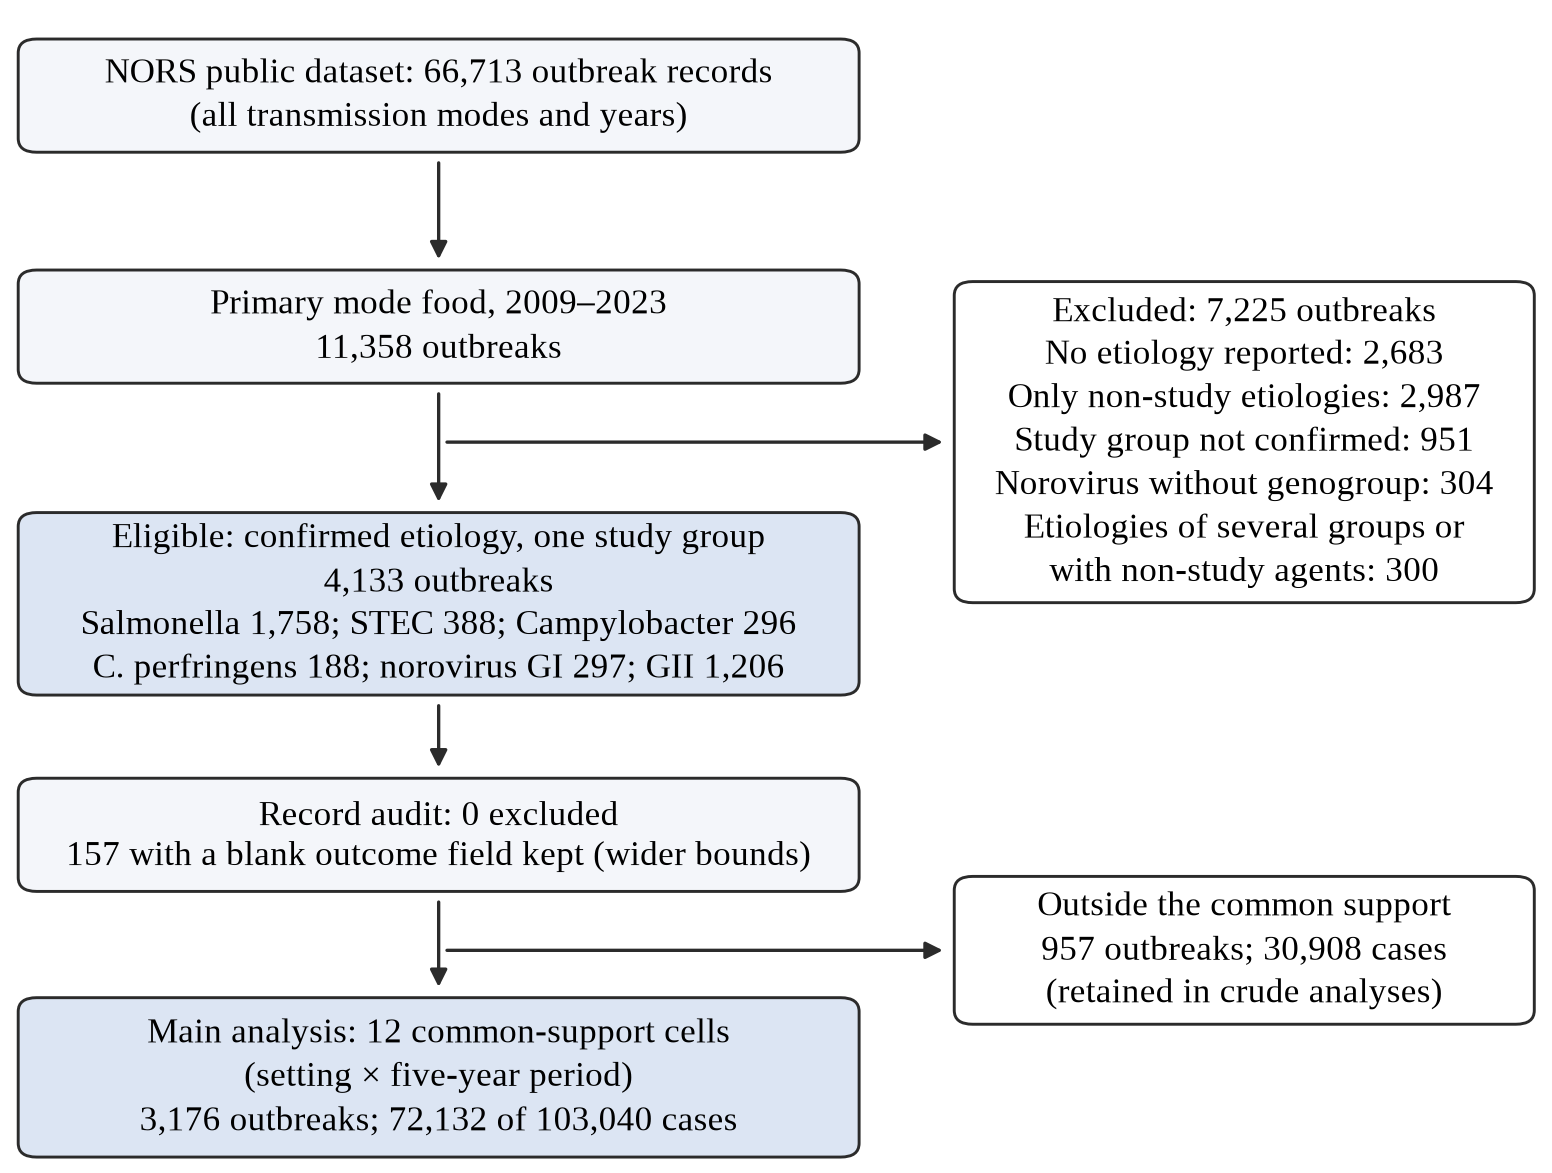
\includegraphics[width=0.82\linewidth]{figures/fig_01_selection_flow.png}
  \caption{Selection of confirmed foodborne outbreaks across six pathogen groups in NORS, United States, 2009--2023. All 157 eligible outbreaks with blank hospitalization fields were retained under logical bounds.}
  \label{fig:flow}
\end{figure}

\subsection{Sample Bounds, Composition-Adjusted Diagnostics and Sensitivity Stress Tests}\label{sec:res-bounds}

Under the 12-cell reference distribution, sample worst-case intervals were 24.7\%--36.8\% for STEC, 14.5\%--31.7\% for \textit{Salmonella}, 7.4\%--19.3\% for \textit{Campylobacter}, 1.3\%--17.2\% for norovirus GII, 0.4\%--19.7\% for \textit{C. perfringens} and 0.4\%--18.7\% for norovirus GI (Table~\ref{tab:group_bounds}; Figure~\ref{fig:intervals}, showing crude $H/C$ and $H/K$ values overlaid). Standardized $\delta = 0$ values lay at 28.5\%, 17.6\%, 8.5\%, 1.6\%, 0.6\% and 0.5\%, respectively. Without assumptions on unrecorded hospitalization outcomes, 4 of 15 pairwise orderings were determined in the sample: STEC exceeded \textit{Campylobacter} (by 5.5 percentage points), \textit{C. perfringens} (5.0 points), norovirus GI (6.0 points) and norovirus GII (7.5 points) (Figure~\ref{fig:verdicts}; Table~\ref{tab:pairwise}). Under illustrative symmetric departures, 14 orderings held at $\delta = 1$ and $2$ points and 12 held at $\delta = 5$ and $10$ points; eight sample-undetermined orderings---STEC above \textit{Salmonella} ($\delta^{*} = 41.3$ points), \textit{Salmonella} above the four lower groups (51.1--81.6) and \textit{Campylobacter} above the lowest three (35.5--37.8)---held across wide bands, whereas all three orderings among norovirus GII, \textit{C. perfringens} and norovirus GI failed below 5 points ($\delta^{*} = 4.2$, $3.7$ and $0.19$ points).

\begin{figure}[!tbp]
  \centering
  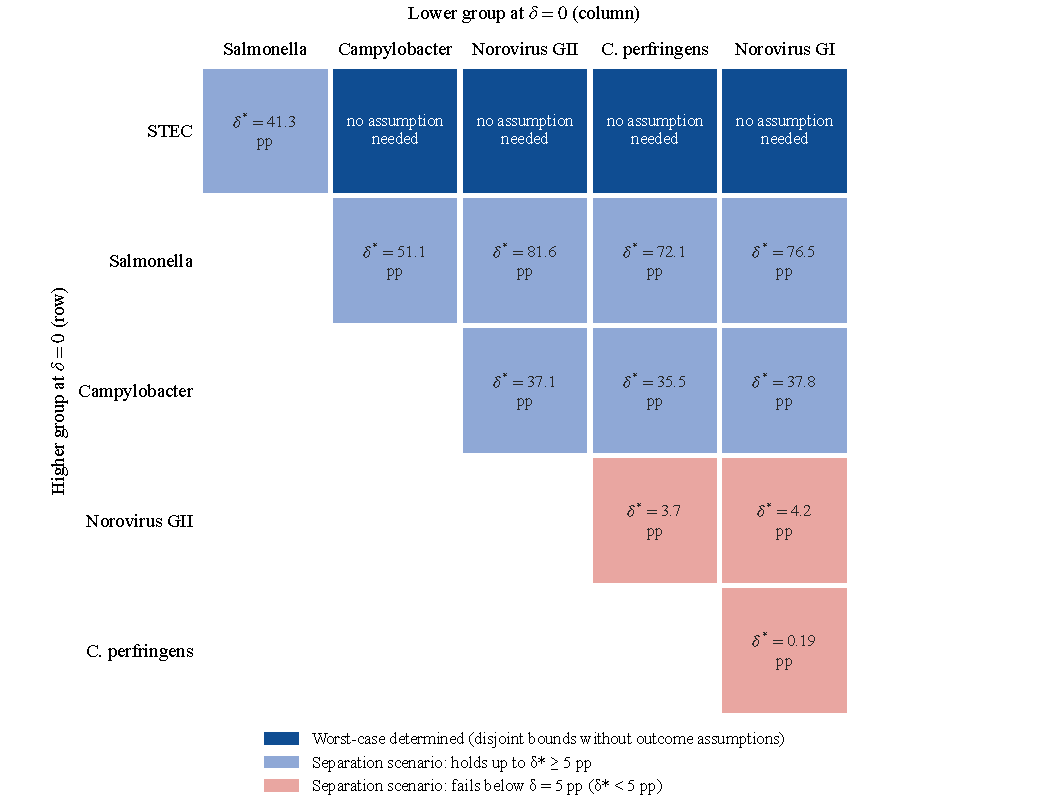
\includegraphics[width=0.80\linewidth]{figures/fig_02_verdict_matrix.pdf}
  \caption{Sample pairwise orderings and critical deviations $\delta^{*}$ across six pathogen groups, NORS foodborne outbreaks, United States, 2009--2023. Dark blue cells hold without assumptions on unrecorded outcomes; light blue and light red cells partition pairs relative to the illustrative scenario threshold $\delta = 5$ percentage points.}
  \label{fig:verdicts}
\end{figure}

\begin{table}[!tbp]
\centering
\scriptsize
\setlength{\tabcolsep}{3pt}
\renewcommand{\arraystretch}{1.12}
\caption{Standardized hospitalization proportion among reported outbreak cases, by pathogen group (12 common-support setting $\times$ period cells, pooled-case reference weights). Sample worst-case intervals are identification intervals; bootstrap ranges are the 2.5th--97.5th percentiles of each bound over 2,000 outbreak-level resamples.}
\label{tab:group_bounds}
\begin{tabular}{>{\raggedright\arraybackslash}p{2.0cm}>{\raggedleft\arraybackslash}p{1.4cm}>{\raggedleft\arraybackslash}p{1.1cm}>{\raggedleft\arraybackslash}p{1.4cm}>{\raggedleft\arraybackslash}p{1.6cm}>{\raggedleft\arraybackslash}p{1.5cm}>{\raggedleft\arraybackslash}p{1.2cm}>{\raggedleft\arraybackslash}p{1.8cm}>{\raggedleft\arraybackslash}p{1.8cm}}
\toprule
Group & Outbreaks & Cases & Unrecorded status (\%) & Worst-case interval (\%) & $\delta$ = 5 interval (\%) & $\delta$ = 0 value (\%) & Bootstrap range of lower bound (\%) & Bootstrap range of upper bound (\%) \\
\midrule
STEC & 268 & 3,943 & 12.7 & 24.7--36.8 & 27.9--29.1 & 28.5 & 21.7--29.3 & 32.6--42.3 \\
Salmonella & 1,277 & 29,151 & 18.1 & 14.5--31.7 & 16.8--18.5 & 17.6 & 13.3--15.9 & 28.2--35.5 \\
Campylobacter & 237 & 2,644 & 14.5 & 7.4--19.3 & 7.9--9.1 & 8.5 & 6.2--9.6 & 14.2--24.4 \\
Norovirus GII & 1,002 & 23,356 & 16.5 & 1.3--17.2 & 1.3--2.4 & 1.6 & 1.1--1.6 & 12.9--20.8 \\
C. perfringens & 147 & 6,568 & 22.2 & 0.4--19.7 & 0.4--1.6 & 0.6 & 0.2--0.9 & 8.5--28.1 \\
Norovirus GI & 245 & 6,470 & 16.2 & 0.4--18.7 & 0.4--1.5 & 0.5 & 0.2--0.6 & 11.7--26.8 \\
\bottomrule
\end{tabular}
\par\smallskip\parbox{0.97\linewidth}{\footnotesize Unrecorded status is the share of retained cases whose hospitalization status was not recorded, including the C $-$ H unrecorded cases from the 52 blank-K records where K was set to H. The $\delta$ = 0 value is the proportion if unrecorded-status cases had the recorded rate of their group and cell.}
\end{table}

\begin{table}[!tbp]
\centering
\scriptsize
\setlength{\tabcolsep}{2.1pt}
\renewcommand{\arraystretch}{1.12}
\caption{Pairwise orderings with worst-case verdicts, critical additive deviations $\delta^{*}$, critical odds-ratio factors $\Gamma^{*}$, illustrative symmetric and asymmetric ($-$15/+5 pp) stress-test verdicts, and bootstrap determination shares.}
\label{tab:pairwise}
\begin{tabular}{>{\raggedright\arraybackslash}p{2.4cm}>{\raggedright\arraybackslash}p{1.55cm}>{\raggedleft\arraybackslash}p{0.92cm}>{\raggedleft\arraybackslash}p{0.95cm}>{\raggedleft\arraybackslash}p{0.6cm}>{\raggedleft\arraybackslash}p{0.6cm}>{\raggedleft\arraybackslash}p{0.6cm}>{\raggedleft\arraybackslash}p{0.65cm}>{\raggedleft\arraybackslash}p{1.1cm}>{\raggedleft\arraybackslash}p{1.4cm}>{\raggedleft\arraybackslash}p{1.4cm}}
\toprule
Ordering at $\delta$ = 0 & Worst case & $\delta^{*}$ (pp) & OR $\Gamma^{*}$ & $\delta$ = 1 & $\delta$ = 2 & $\delta$ = 5 & $\delta$ = 10 & Asym ($-$15/+5) & Boot det., worst (\%) & Boot det., $\delta$ = 5 (\%) \\
\midrule
STEC $>$ CAMP & determined & $\infty$ & $\infty$ & yes & yes & yes & yes & yes & 97.0 & 100.0 \\
STEC $>$ CPERF & determined & $\infty$ & $\infty$ & yes & yes & yes & yes & yes & 91.6 & 100.0 \\
STEC $>$ NoV GI & determined & $\infty$ & $\infty$ & yes & yes & yes & yes & yes & 93.6 & 100.0 \\
STEC $>$ NoV GII & determined & $\infty$ & $\infty$ & yes & yes & yes & yes & yes & 100.0 & 100.0 \\
SAL $>$ NoV GII & undetermined & 81.6 & 342.1 & yes & yes & yes & yes & yes & 14.2 & 100.0 \\
SAL $>$ NoV GI & undetermined & 76.5 & 1420.4 & yes & yes & yes & yes & yes & 14.5 & 100.0 \\
SAL $>$ CPERF & undetermined & 72.1 & $\infty^{\dagger}$ & yes & yes & yes & yes & yes & 24.8 & 100.0 \\
SAL $>$ CAMP & undetermined & 51.1 & 17.5 & yes & yes & yes & yes & yes & 4.2 & 100.0 \\
STEC $>$ SAL & undetermined & 41.3 & 8.41 & yes & yes & yes & yes & yes & 0.6 & 100.0 \\
CAMP $>$ NoV GI & undetermined & 37.8 & 115.9 & yes & yes & yes & yes & yes & 0.1 & 98.4 \\
CAMP $>$ NoV GII & undetermined & 37.1 & 41.2 & yes & yes & yes & yes & yes & 0.0 & 100.0 \\
CAMP $>$ CPERF & undetermined & 35.5 & 120.6 & yes & yes & yes & yes & yes & 1.8 & 100.0 \\
NoV GII $>$ NoV GI & undetermined & 4.2 & 7.75 & yes & yes & no & no & no & 0.0 & 35.2 \\
NoV GII $>$ CPERF & undetermined & 3.7 & 4.99 & yes & yes & no & no & no & 0.0 & 33.1 \\
CPERF $>$ NoV GI & undetermined & 0.19 & 1.19 & no & no & no & no & no & 0.0 & 0.0 \\
\bottomrule
\end{tabular}
\par\smallskip\parbox{0.97\linewidth}{\footnotesize Boot det. columns show the percentage of 2,000 bootstrap replicates in which the ordering is determined (non-overlapping intervals) at worst case and $\delta$ = 5 pp. $^{\dagger}$OR $\Gamma^{*}$ = $\infty^{\dagger}$ for SAL $>$ CPERF reflects 9/72 cells having zero recorded hospitalizations (p\_js = 0), which pure multiplicative scaling cannot shift upward; applying a 0.1\% continuity floor yields $\Gamma^{*}$ = 955.7 (Table S4).}
\end{table}


\begin{figure}[!tbp]
  \centering
  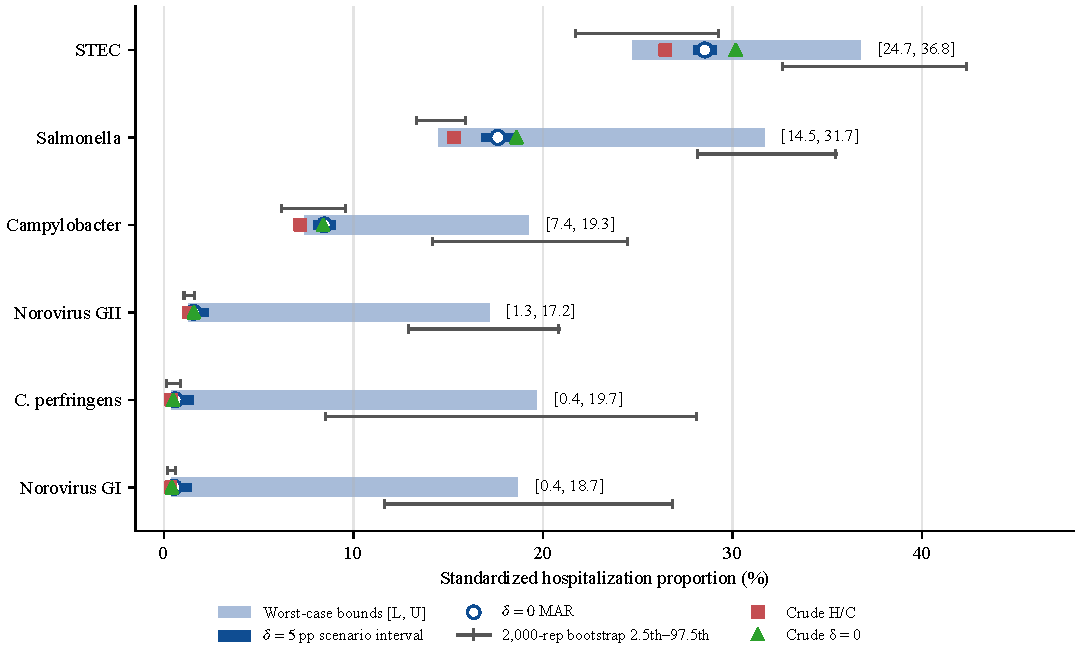
\includegraphics[width=0.92\linewidth]{figures/fig_03_bound_intervals.pdf}
  \caption{Standardized hospitalization proportions and identification intervals overlaid with crude $H/C$ (squares) and $H/K$ (triangles) conventions across the 12 common-support cells. Light bars show worst-case intervals; dark bars show the $\delta = 5$ percentage-point scenario; error bars give 2.5th--97.5th percentiles over 2,000 outbreak-level bootstrap replicates.}
  \label{fig:intervals}
\end{figure}

Comparing partially recorded ($M_i > 0, K_{\text{rec},i} > 0$) against fully recorded ($M_i = 0$) outbreaks demonstrated that large crude differences reflect outbreak composition rather than uniform outcome-dependent missingness (Supplementary Table S4). Partially recorded outbreaks were substantially larger (median 16 vs.\ 5 cases for STEC; 19 vs.\ 7 for \textit{Salmonella}) and far more often multistate (60.0\% vs.\ 11.7\% for STEC; 34.2\% vs.\ 2.4\% for \textit{Salmonella}). After cell standardization, the STEC partial-minus-full gap collapsed from $+10.93$ points to $+0.19$ points (and actually reversed within multistate outbreaks to $-1.28$ points, leaving ``Std obs $-$ Full'' $= -3.22$ points because the main $\delta=0$ anchor of 28.5\% lay below the standardized fully recorded STEC rate of 31.1\%). For \textit{Salmonella}, a $+9.02$-point within-cell difference persisted (``Std obs $-$ Full'' $= +2.86$ points) and was strongest within multistate outbreaks ($+11.98$ points vs.\ $+4.34$ single-state), coinciding with active subtype-linked surveillance rather than solely outcome-selective field recording. In 11 low-missingness states ($<5\%$ unrecorded status), recorded rates were 26.2\% (STEC), 13.0\% (\textit{Salmonella}), 8.8\% (\textit{Campylobacter}), 1.3\% (norovirus GII), 0.0\% (\textit{C. perfringens}) and 0.3\% (norovirus GI). Scenario stress tests confirmed that all 12 upper-tier orderings remain separated under asymmetric bands of $-10/+5$, $-15/+5$ and $-20/+5$ points (Figure~\ref{fig:cal2d}; Table~\ref{tab:pairwise}). Under odds-ratio scaling, 14 of 15 pairs held at $\Gamma \le 3.0$ and 13 at $\Gamma = 5.0$ both under pure multiplicative scaling and after imposing a 0.1\% continuity floor on all 9 zero-rate cells ($\Gamma^{*} = 8.41$ for STEC above \textit{Salmonella}; $\Gamma^{*} = 955.7$ vs.\ $\infty^{\dagger}$ for \textit{Salmonella} above \textit{C. perfringens}).

\begin{figure}[!tbp]
  \centering
  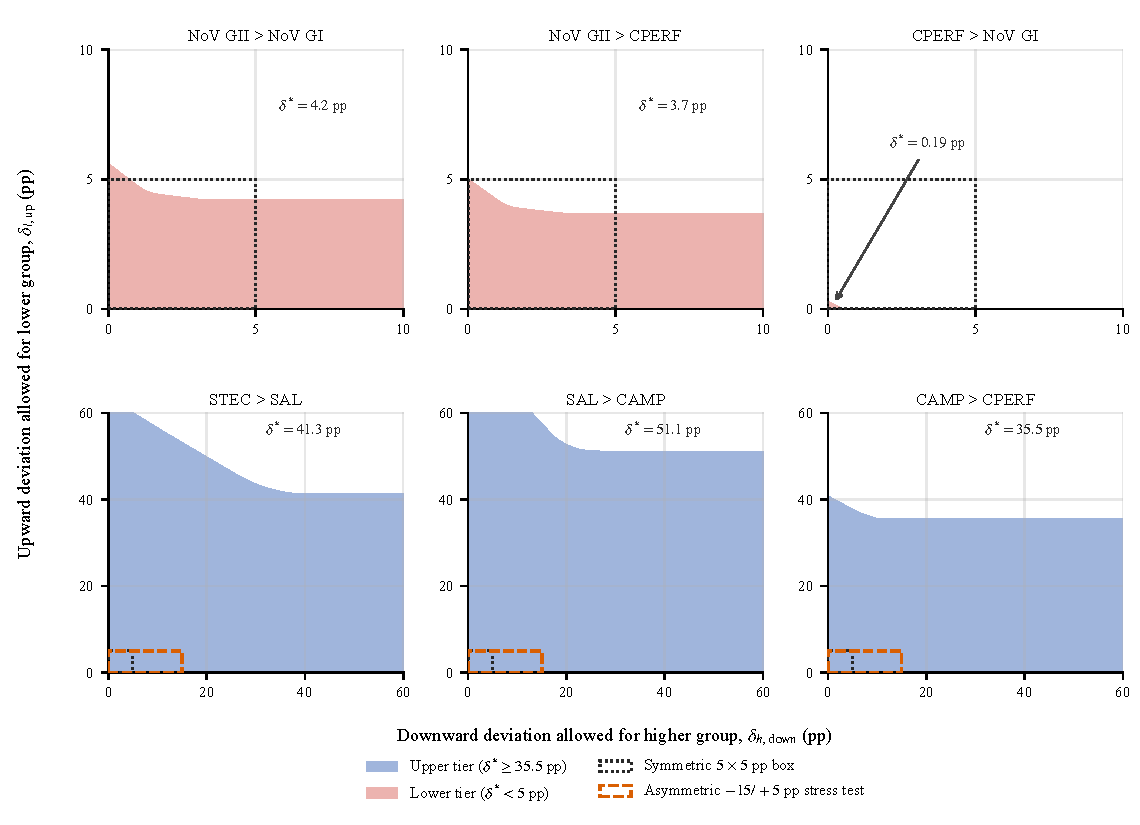
\includegraphics[width=0.95\linewidth]{figures/fig_04_calibrated_2d.pdf}
  \caption{Two-dimensional asymmetric sensitivity across all 15 pathogen pairs (higher group at $\delta = 0$ first). Shaded regions denote combinations of downward deviation allowed for the higher group ($\delta_{h,\text{down}}$) and upward deviation allowed for the lower group ($\delta_{l,\text{up}}$) preserving separation. Dotted and dashed boxes illustrate the symmetric $5 \times 5$ pp and asymmetric $-15/+5$ pp scenario stress tests.}
  \label{fig:cal2d}
\end{figure}

\subsection{30-Hypothesis Inference, State Clustering, Calibration and Rank Sets}\label{sec:res-inference}

High single-outbreak concentration explained skewed upper-bound sampling variance (Supplementary Table S7): maximum stratum case shares reached 69.2\% for \textit{C. perfringens} (max HHI $0.501$, $N_{\text{eff}} = 2.00$), 62.1\% for norovirus GI ($0.508$, $N_{\text{eff}} = 1.97$), 65.5\% for \textit{Campylobacter} ($0.491$, $N_{\text{eff}} = 2.04$) and 63.3\% for STEC ($0.479$, $N_{\text{eff}} = 2.09$) versus 33.0\% for \textit{Salmonella} ($0.133$, $N_{\text{eff}} = 7.49$). Across 33 states with $\ge 500$ common-support cases, unrecorded status spanned 0.0\%--40.3\% (median 12.2\%), and the top three states held 91.4\% of unrecorded STEC cases, 65.1\% for \textit{Salmonella} and 63.4\% for \textit{C. perfringens}; 53-state clustering scaled lower-difference SEs by factors of 0.77 to 1.73 (largest for STEC vs.\ \textit{Salmonella}, $1.73$).

Across all 30 ordered two-sided hypotheses (Table~\ref{tab:joint_inference}; Figure~\ref{fig:inference_followup}a), STEC above norovirus GII remained statistically significant without unrecorded-outcome assumptions under every inferential procedure: outbreak-HC1 Gaussian Max-$T$ ($c_{\text{sim},30} = 2.611$, $p_{\text{FWER}} = 0.0245$, IM 95\% CI $[+3.2, +39.2]$ pp), 2,000-replicate bootstrap covariance Gaussian Max-$T$ ($c = 2.617$, $p = 0.0315$), 53-state clustering ($c = 2.536$, $p = 0.0332$, state IM 95\% CI $[+2.9, +44.5]$ pp), 53-state wild cluster bootstrap ($p_{\text{WCB}} = 0.0306$), and studentized non-Gaussian bootstrap Max-$T$ ($c_{\text{boot}} = 2.725$, $p = 0.0430$). Under the $\delta = 5$ pp band ($c_{\text{sim},30} = 2.730$ HC1, $2.683$ state, $2.899$ non-Gaussian bootstrap), all 12 upper-tier orderings were jointly significant across Gaussian HC1 ($p < 0.001$), 53-state ($p < 0.001$), WCB ($p \le 0.0002$), and studentized non-Gaussian bootstrap Max-$T$ (maximum $p = 0.0020$ for \textit{Campylobacter} above norovirus GI; $p \le 0.0010$ for the other 11 pairs). Under the asymmetric $-15/+5$ pp band, all 12 upper-tier orderings likewise remained jointly significant under both HC1 and 53-state 30-hypothesis FWER ($p \le 0.0001$). Using dynamic $c_{\text{sim},30}(\delta)$, simultaneous 95\% confidence tipping points were $\infty$ for STEC above norovirus GII, 73.2--80.6 pp (HC1) / 77.3--90.3 pp (state) for STEC vs.\ \textit{Campylobacter}, \textit{C. perfringens} and norovirus GI, and 18.5--57.7 pp (HC1) / 18.0--54.7 pp (state) for the other upper-tier pairs ($\le 1.3$ pp for bottom three).

Simultaneous 95\% rank confidence sets across all five worst-case procedures yielded $[1, 5]$ for STEC, $[2, 6]$ for norovirus GII, and $[1, 6]$ for the remaining four groups. Under both $\delta = 5$ pp and the asymmetric $-15/+5$ pp scenario, the joint 95\% rank sets separated STEC $[1, 1]$, \textit{Salmonella} $[2, 2]$ and \textit{Campylobacter} $[3, 3]$ from the indistinguishable lower tier $[4, 6]$ across every inferential method.

In the 500-replicate bootstrap-world calibration preserving $n_{js}$ (Supplementary Table S8), asymptotic HC1 under-covered in sparse $N_{\text{eff}} \approx 2$ strata (IM 95\% empirical boundary coverage 76.4\% min, 87.4\% median; ratio of mean HC1 SE to MC SD 0.754--1.024). Empirical 30-hypothesis FWER rejection rates at nominal 5\% were: 32.8\% (HC0), 29.8\% (HC1), 25.6\% (non-Gaussian bootstrap critical value), 21.4\% (53-state clustering) and 20.6\% (wild cluster bootstrap) under worst-case bounds, falling to 20.8\%, 18.0\%, 12.6\%, 8.8\% and 8.0\% at $\delta = 5$ pp. Thus, accounting for state correlation and skewness improves calibration substantially, though anti-conservative finite-sample error persists in sparse highly concentrated strata.

\begin{table}[!tbp]
\centering
\scriptsize
\setlength{\tabcolsep}{2.3pt}
\renewcommand{\arraystretch}{1.12}
\caption{Joint M-estimation inference for the 15 pairwise standardized differences combining outbreak-HC1 and 53-state-clustered sandwich covariances, Imbens--Manski 95\% CIs, 200,000-draw Gaussian multiplier Max-T FWER p-values, and dynamic simultaneous 95\% confidence tipping points.}
\label{tab:joint_inference}
\begin{tabular}{>{\raggedright\arraybackslash}p{2.4cm}>{\raggedleft\arraybackslash}p{1.95cm}>{\raggedleft\arraybackslash}p{2.05cm}>{\raggedleft\arraybackslash}p{2.2cm}>{\raggedleft\arraybackslash}p{2.2cm}>{\raggedleft\arraybackslash}p{1.05cm}>{\raggedleft\arraybackslash}p{2.25cm}}
\toprule
Ordering at $\delta$ = 0 & ID bounds (pp) & IM 95\% CI (pp) & HC1 FWER p (w / $\delta$=5) & State FWER p (w / $\delta$=5) & $\delta^{*}$ (pt) & 95\% $\delta^{*}$ (HC1 / State) \\
\midrule
STEC $>$ CAMP & [+5.5, +29.3] & [+0.2, +33.3] & 0.260 / <0.001 & 0.115 / <0.001 & $\infty$ & 75.4 / 83.9 \\
STEC $>$ CPERF & [+5.0, +36.4] & [-2.5, +40.1] & 0.572 / <0.001 & 0.518 / <0.001 & $\infty$ & 76.6 / 78.2 \\
STEC $>$ NoV GI & [+6.0, +36.3] & [-1.0, +40.1] & 0.393 / <0.001 & 0.186 / <0.001 & $\infty$ & 82.2 / 91.2 \\
STEC $>$ NoV GII & [+7.5, +35.4] & [+3.2, +39.2] & 0.018 / <0.001 & 0.027 / <0.001 & $\infty$ & $\infty$ / $\infty$ \\
SAL $>$ NoV GII & [-2.7, +30.4] & [-6.3, +33.6] & 1.000 / <0.001 & 1.000 / <0.001 & 81.6 & 58.6 / 55.4 \\
SAL $>$ NoV GI & [-4.2, +31.3] & [-10.7, +34.5] & 1.000 / <0.001 & 1.000 / <0.001 & 76.5 & 48.3 / 50.4 \\
SAL $>$ CPERF & [-5.2, +31.3] & [-12.3, +34.6] & 1.000 / <0.001 & 1.000 / <0.001 & 72.1 & 45.0 / 43.6 \\
SAL $>$ CAMP & [-4.7, +24.2] & [-9.4, +27.8] & 1.000 / <0.001 & 1.000 / <0.001 & 51.1 & 21.5 / 19.3 \\
STEC $>$ SAL & [-7.0, +22.2] & [-11.1, +26.0] & 1.000 / <0.001 & 1.000 / <0.001 & 41.3 & 20.1 / 20.6 \\
CAMP $>$ NoV GI & [-11.2, +18.8] & [-17.9, +23.4] & 1.000 / <0.001 & 1.000 / <0.001 & 37.8 & 20.9 / 22.1 \\
CAMP $>$ NoV GII & [-9.7, +17.9] & [-13.4, +22.5] & 1.000 / <0.001 & 1.000 / <0.001 & 37.1 & 21.3 / 20.8 \\
CAMP $>$ CPERF & [-12.2, +18.9] & [-19.5, +23.4] & 1.000 / <0.001 & 1.000 / <0.001 & 35.5 & 19.2 / 18.6 \\
NoV GII $>$ NoV GI & [-17.4, +16.8] & [-23.9, +20.2] & 1.000 / 0.931 & 1.000 / 0.938 & 4.2 & 1.5 / 1.5 \\
NoV GII $>$ CPERF & [-18.4, +16.8] & [-25.5, +20.2] & 1.000 / 0.963 & 1.000 / 0.962 & 3.7 & 1.0 / 1.0 \\
CPERF $>$ NoV GI & [-18.3, +19.3] & [-24.8, +26.4] & 1.000 / 1.000 & 1.000 / 1.000 & 0.19 & 0.00 / 0.00 \\
\bottomrule
\end{tabular}
\par\smallskip\parbox{0.97\linewidth}{\footnotesize Outbreak-HC1 critical values: c\_sim = 2.49 (worst case), 2.53 ($\delta$ = 5); state-clustered: 2.46 / 2.49 (wild cluster bootstrap STEC $>$ NoV GII p = 0.028). 95\% $\delta^{*}$ uses dynamic c\_sim($\delta$). Simultaneous 95\% rank confidence sets at $\delta$ = 5: STEC [1,1]; SAL [2,2]; CAMP [3,3]; NoV GII [4,6]; CPERF [4,6]; NoV GI [4,6] (worst case: STEC [1,5], NoV GII [2,6], others [1,6]).}
\end{table}


\begin{figure}[!tbp]
  \centering
  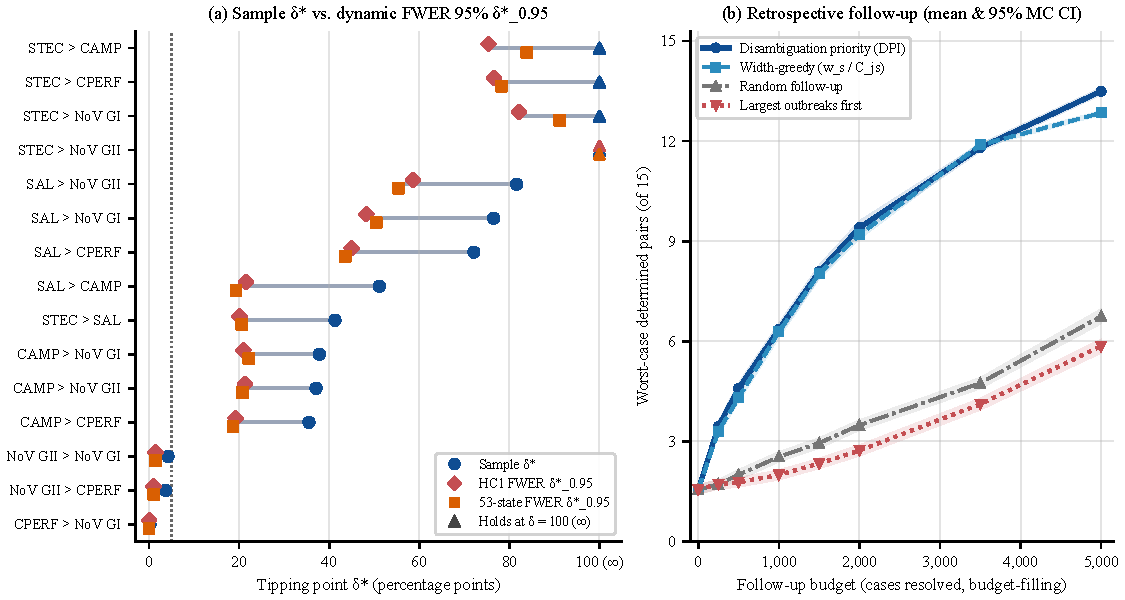
\includegraphics[width=0.96\linewidth]{figures/fig_05_inference_followup.pdf}
  \caption{Simultaneous 30-hypothesis confidence tipping points and cost-conditional follow-up benchmarks. (a) Sample tipping point $\delta^{*}$ versus dynamic 30-hypothesis FWER 95\% tipping points $\delta^{*}_{0.95}$ under outbreak-HC1 and 53-state clustering. (b) Per-case cost model (budget in cases resolved, budget-filling). (c) Per-outbreak cost model (budget in outbreaks contacted), illustrating strategy reversal between per-case and per-outbreak costs and unified optimality of Eq.~\ref{eq:followup}.}
  \label{fig:inference_followup}
\end{figure}

\subsection{Cost-Conditional Follow-Up Benchmarks and Sensitivity Variants}\label{sec:res-voi}

Evaluating Eq.~\ref{eq:followup} across 200 budget-filling masking trials on 2,414 fully recorded outbreaks (45,249 cases; baseline mean 1.55 determined pairs) revealed a sharp dependence on follow-up cost structure (Figure~\ref{fig:inference_followup}b--c; Supplementary Table S10). Under a per-case cost budget (1,000 cases), per-case stratum leverage $w_s/C_{js}$ resolved 6.29 pairs (95\% CI $[6.09, 6.48]$), more than doubling random follow-up (2.54 pairs, $[2.38, 2.69]$) and tripling largest-outbreak-first (2.00 pairs, $[1.84, 2.15]$; mean leverage $0.0088$ vs.\ $0.0573$ pp/case). Conversely, under a per-outbreak cost budget (100 outbreaks contacted), largest-outbreak-first reversed rank and strongly beat both random follow-up (7.90 vs.\ 3.27 pairs) and per-case $w_s/C_{js}$ (7.38 pairs), while the cost-optimal per-outbreak width rule $w_s U_i/C_{js}$ dominated all strategies (9.12 pairs, $[9.00, 9.23]$ at 100 outbreaks; 6.41 vs.\ 1.92--4.01 at 25 outbreaks). Under a mixed cost model ($\text{cost}_i = 20 + U_i$ case-equivalents; Supplementary Figure S3a), mixed cost-normalized targeting achieved the highest resolution at 1,000 units (4.09 pairs vs.\ 3.73 per-case, 3.57 per-outbreak, 1.95 largest-first, 1.94 random) and 2,000 units (6.24 vs.\ 4.74–5.05). Supplementary sensitivity checks confirm that heuristic DPI adds $+0.07$ pairs (95\% CI $[-0.07, +0.21]$) over $w_s/C_{js}$ in single-shot ranking, improves under 250-case adaptive tranches (7.31 at 1,000 cases), and preserves gains under MNAR, state-clustered, and 70\%-yield masking (Supplementary Figure S3b; real-data strata ranked in Supplementary Table S11; descriptive worst-case width decomposition in Supplementary Table S9).

Across all 17 cohort and specification sensitivity variants (Supplementary Table S5; Supplementary Figure S2), 4 to 7 pairs held without unrecorded-outcome assumptions and 12 to 14 at $\delta = 5$ pp, with zero reversals among the four primary pairs and only five variants (R1a, R2, R4a, R5, R6b) shifting a single low-tier $\delta = 0$ direction. Restricting exclusively to the 3,659 single-state outbreaks (variant R11) kept the identical 12 common-support cells, 4 worst-case pairs and 12 $\delta = 5$ pairs (zero changes vs.\ main). Including suspected etiologies (R8; 5,084 outbreaks, 16 cells) gave 5 / 13 pairs; excluding 79 healthcare outbreaks (R9) gave 4 / 12 (zero changes); and equal outbreak-level within-cell weighting (R10) gave 7 / 14 (zero reversals). Bootstrap resampling (Table~\ref{tab:pairwise}; Supplementary Table S6) determined the four primary worst-case orderings in 91.6\%--100.0\% of replicates ($0/2,000$ replicates lacked $K_{\text{rec}}$).

\section{Discussion}\label{sec:discussion}

By combining nonparametric partial identification, composition-adjusted missingness diagnostics, 30-hypothesis FWER inference and cost-conditional follow-up benchmarks, this study delineates what CDC NORS foodborne outbreak records establish robustly from what depends on missing-data assumptions, case ascertainment and finite-sample error. Without assumptions on unrecorded hospitalization outcomes, 4 of 15 sample orderings separate and STEC above norovirus GII remains significant across all 30 two-sided tests under every inferential check ($p = 0.024$ outbreak-HC1; $p = 0.031$ bootstrap covariance; $p = 0.033$ 53-state clustering; $p = 0.031$ wild cluster bootstrap; $p = 0.043$ non-Gaussian studentized bootstrap). High stratum concentration ($\text{HHI} \approx 0.50$, $N_{\text{eff}} \approx 2.0$ in sparse strata) inflates upper-bound variance for \textit{C. perfringens} and norovirus GI, leaving simultaneous worst-case ranks at $[1, 5]$ for STEC, $[2, 6]$ for norovirus GII and $[1, 6]$ for the remaining pathogens.

Commonly reported denominator conventions map onto specific slices of our framework: dividing hospitalizations by all ill persons ($H/C$) matches worst-case lower bounds $L_j$~\cite{cdc2026surveillance2019,heiman2015escherichia}, whereas dividing by persons with known status ($H/K$) approximates the within-cell missing-at-random anchor ($\delta = 0$)~\cite{burke2019norovirus,wikswo2022enteric}. In comparison with US national burden estimates by Scallan et al.~\cite{scallan2011foodborne} (updated for 2019 in~\cite{scallanwalter2025foodborne}) and prior NORS summaries~\cite{deweymattia2018surveillance}, our standardized $\delta = 0$ proportions for STEC (28.5\%), \textit{Salmonella} (17.6\%) and \textit{Campylobacter} (8.5\%) fall below their proportions among laboratory-confirmed bacterial illnesses (46.2\% for O157 STEC, 27.2\% for \textit{Salmonella} and 17.1\% for \textit{Campylobacter}, reflecting broader non-O157 STEC inclusion and NORS setting standardization), while matching \textit{C. perfringens} (0.6\% vs.\ 0.6\% derived from outbreak data). For norovirus, however, Scallan et al.\ estimate only 0.03\% hospitalizations per total estimated community illness, whereas NORS outbreak-reported proportions are roughly 50-fold higher (1.6\% for norovirus GII at $\delta = 0$): milder viral gastroenteritis outbreaks seldom reach public health surveillance unless severe cases trigger investigation. Across all three lowest-risk agents, worst-case ambiguity (15.9--19.3 points) exceeds 1 percentage-point differences, rendering their internal ordering unresolvable ($\delta^{*} = 0.19$--$4.2$ points)~\cite{vega2014genotypic,grass2013epidemiology,burke2019norovirus}. Discarding the 157 incomplete records (variant R3b) would overstate sample worst-case orderings (7 vs.\ 4) by changing the estimand to omit ambiguous records.

Crucially, stratified checks clarify why crude comparisons between partially and fully recorded outbreaks must be interpreted cautiously. Although crude known-status hospitalization was higher in partially recorded outbreaks for STEC and \textit{Salmonella} and tracked rates in the 11 low-missingness states to fully recorded levels (26.2\% STEC; 13.0\% \textit{Salmonella}), this gap was largely confounded by outbreak size and multistate laboratory surveillance: within cells, the STEC gap vanished ($+0.19$ points; ``Std obs $-$ Full'' $= -3.22$ points). Thus, the data do not establish a uniform direction of residual missingness departure. Nevertheless, all 12 upper-tier orderings remain robustly separated across $\pm 5$-point symmetric bands, $-15/+5$ to $-20/+5$ asymmetric stress tests, and odds-ratio factors up to $\Gamma = 3.0$ (14 of 15 total pairs including two lower-tier pairs at $\Gamma = 3.0$; 12 upper-tier pairs throughout $\Gamma \le 5.0$). Simultaneous 95\% rank sets computed at worst case, $\delta = 5$ points and $-15/+5$ points identically separate STEC $[1, 1]$, \textit{Salmonella} $[2, 2]$ and \textit{Campylobacter} $[3, 3]$ from the lower tier $[4, 6]$ whenever departure bounds hold at those scenarios.

Operational follow-up triage depends critically on how agencies incur verification costs. Targeting follow-up by stratum leverage $w_s/C_{js}$ dominates when costs scale per case resolved, whereas targeting by outbreak width $w_s U_i/C_{js}$ dominates when contacting a jurisdiction carries a fixed per-outbreak cost (under which targeting largest outbreaks also beats random selection). Framing prioritization around expected bound reduction per unit cost resolves this apparent reversal transparently across all cost regimes.

\subsection{Limitations}\label{sec:limitations}

First, NORS reporting is voluntary and overall outbreak reporting rates vary four-fold between high- and low-reporting states (spanning roughly 5 to 86 outbreaks per 10 million population annually, and $>40$-fold for norovirus)~\cite{white2022foodborne}. Second, partial-identification bounds take estimated case counts $C_i$ (as well as $H_i$ and $K_i$) as accurate; differential case ascertainment between laboratory-confirmed multistate clusters (common in STEC and \textit{Salmonella}) and complaint-detected local outbreaks can bias rates by lowering detected mild illnesses~\cite{heiman2015escherichia}, though restricting entirely to single-state outbreaks (variant R11) preserved every main verdict. Third, common support was selected data-dependently ($\ge 3$ outbreaks per group), dropping 30.0\% of cases and placing 90.4\% of pooled weight in 2009--2018 because only restaurants met support criteria in 2019--2023 (9.6\%); retrospective follow-up of 2009--2018 records is practically infeasible, so our follow-up simulation applies prospectively to ongoing surveillance. Fourth, the masking cohort of fully recorded outbreaks is smaller and more often single-state than partially recorded targets. Fifth, outbreak-versus-sporadic hospitalization comparability in Ebel et al.~\cite{ebel2016comparing} pertains strictly to laboratory-confirmed FoodNet bacterial infections (\textit{Salmonella}, O157 STEC, \textit{Campylobacter}, \textit{Listeria}) and not non-O157 STEC, \textit{C. perfringens} or norovirus; our genus-level estimand lacks age/comorbidity covariates and pools distinct serotypes and subtypes~\cite{jones2008salmonellosis,gould2013increased,geissler2017increasing}. Sixth, bootstrap-world calibration showed anti-conservative 30-test rejection rates for asymptotic HC1 in sparse strata ($N_{\text{eff}} \approx 2$), and wildly unequal state cluster sizes (3 states holding 91.4\% of unrecorded STEC cases) can cause wild cluster bootstrap tests to slightly over-reject~\cite{mackinnon2017wild}.

\subsection{Conclusions}\label{sec:conclusions}

In US foodborne outbreak surveillance (2009--2023, predominantly weighted to 2009--2018), STEC exhibits a higher standardized hospitalization proportion than norovirus GII without unrecorded-outcome assumptions across all 30 two-sided tests and five inferential procedures. Under $\delta = 5$ percentage points or asymmetric $-15/+5$ percentage-point stress tests, all 12 upper-tier orderings hold jointly and yield simultaneous 95\% rank sets separating STEC $[1,1]$, \textit{Salmonella} $[2,2]$ and \textit{Campylobacter} $[3,3]$ from the lower tier $[4,6]$, whereas orderings among \textit{C. perfringens}, norovirus GI and norovirus GII remain unresolved. Surveillance comparisons should accompany reported hospitalization proportions with partial-identification bounds and joint rank confidence sets, and agencies prioritizing follow-up verification should target expected bound reduction per unit cost ($w_s U_i / (C_{js}\,\text{cost}_i)$) tailored to their operational cost structure.

\clearpage
\section*{Author Contributions}\label{sec:contributions}
\markboth{Declarations}{Declarations}

C.W. conceived the study, curated the CDC NORS data snapshot, designed and implemented the statistical methodology and reproducibility pipeline, generated all tables and figures, and wrote and revised the manuscript.

\section*{Funding}\label{sec:funding}

This study received no specific grant from any funding agency in the public, commercial or not-for-profit sectors.

\section*{Competing Interests}\label{sec:competing}

The author declares no competing financial or non-financial interests.

\section*{Use of Automated Tools}\label{sec:ai}

Large language model coding and editing assistants were used during software engineering, LaTeX typesetting, and language polishing. The author independently verified all mathematical derivations, statistical implementations, data outputs, and scientific interpretations.

\section*{Data and Code Availability}\label{sec:availability}

The NORS public dataset is available from the CDC open data portal~\cite{cdc2024norsdata}. The dated extract (\texttt{nors\_soda\_full\_20261125T040830Z.csv}, SHA-256 pinned), derived cohorts, excluded-outbreak audit summaries, analysis results JSON, all 14 CSV/LaTeX tables, and replication scripts are archived with this release. Rerunning \texttt{reproduce.py} from the raw extract reproduces all deterministic bounds, cohorts, and formatted non-bootstrap CSV tables identically, matches 2,000-replicate bootstrap distributions within Monte Carlo tolerance, verifies identical 30-hypothesis rejection decisions, and reproduces numerical simulation quantities to within deterministic ($\le 10^{-9}$) or cross-platform BLAS ($\le 10^{-3}$; at most $\approx 0.025$ in rare Gaussian-tail quantiles) tolerance without altering any published table entry.

\section*{Ethics}\label{sec:ethics}

The analysis used only publicly released outbreak-level counts; no individual-level or identifiable data were accessed.


\FloatBarrier
\clearpage
{\small
\bibliographystyle{unsrtnatclean}
\bibliography{bibliography}
}

\end{document}
